\section{Experiments}
\label{sec:experiments}

To validate our method, we performed experiments on two datasets: one is the synthetic half-moons dataset, and the other is the real-world Pascal VOC 2012 dataset.

\subsection{Experiments on the half-moons dataset}
\label{subsec:half-moons}

Here we give the details of the half-moons experiment discussed in the Introduction section. We use the half-moons dataset provided by Scikit learn \citep{scikit-learn} to generate 10,000 points with a Gaussian noise of $\mathcal{N}(0, 0.2)$. The dataset is split into 8,000 training points and 2,000 testing ones. The model used is an MLP.

We measure two indicators of performance for each attribution method: a lack of artifacts not reflecting the model's behaviour, and a low variation of attributions between close points. To that goal, we use two metrics, \textbf{purity} and \textbf{standard deviation}, defined in the following way. We know that a well-trained model should classify about half of the data points as upper moon, class $1$, and the other half as lower moon, class $0$. Such a model should consider both features of each point important for the classification into class $1$. Therefore, for such a model, we expect in a good attribution method, the top $50\%$ points as ranked by the quantity $\widetilde{attr}(\textbf{x}; f) = \sum_{i=0}^1 |attr_i(\textbf{x}; f)|$, to be classified as $1$ (assuming the baseline is chosen as a point to which the network gives a near-zero score). With this in mind, purity is defined as
\begin{equation}
\begin{split}
    \textrm{Purity} &= \frac{1}{N/2}\sum_{\textbf{x}, \, \widetilde{attr}(\textbf{x}; f) \in \textrm{Top 50\% of all attr}} \textrm{argmax}(f(\textbf{x})),
\end{split}
\label{eq:moons-purity}
\end{equation}
where $N$ is the number of data points. We see that this is the average value of the predicted class labels for half of the points. From the above, we infer that, for a well-trained model, we prefer an attribution method that results in the purity close to $1$. In contrast, a random attribution method in this case would result in the purity score of $0.5$. 

For the second metric, standard deviation, points that belong to the same moon to have similar $\widetilde{attr}(\textbf{x}; f)$. Therefore, define
\begin{equation}
\begin{split}
    \textrm{Std}_i &= \textrm{std}\{\widetilde{attr}(\textbf{x}; f), \, \textrm{argmax}(f(\textbf{x})) \in \textrm{Moon }_i\}.
\end{split}
\label{eq:moons-std}
\end{equation}
We expect this standard deviation metric to be low for the points belonging to either class. 

In this experiment, we compare the results of attributions from Geodesic IG with the original IG, as well as more recent comparable methods including Enhanced IG \citep{jha2020enhanced}, GradientShap \citep{lundberg2017unified}, SmoothGrad \citep{smilkov2017smoothgrad}.

For all of the methods, we use $(-0.5, -0.5)$ as a baseline. Enhanced IG is an improvement over IG where the kNN algorithm is used to avoid computing gradients on paths on out of sample distributions. The chosen number of neighbours for the kNN part of both Enhanced IG and Geodesic IG is $5$. We perform an ablation study of this parameter in Appendix \ref{app:half-moons}. 

\begin{table}[t]
	\centering
	\resizebox{0.48\textwidth}{!}{%
	\begin{tabular}{lccc}
		\toprule
		\textbf{Method} & Purity $\uparrow$ & $\textrm{STD}_0$ $\downarrow$ & $\textrm{STD}_1$ $\downarrow$ \\
		\midrule
        GradientShap    & 0.761 (0.158)   & 1.90 (0.520)  & 5.01 (0.581) \\
		IG              & 0.802 (0.142)  & 1.44 (0.139) & 4.915 (0.574)  \\
        SmoothGrad      & 0.800 (0.142)  &  1.42 (0.139) & 4.720 (0.649)  \\
        Enhanced IG     & 0.738 (0.209)  &  1.23 (0.229) & 1.876 (1.10) \\
		\midrule
		Geodesic IG     & \textbf{0.978} (0.0143)  & \textbf{0.237} (0.0278) & \textbf{0.267} (0.129) \\
		\bottomrule
	\end{tabular}%
	}
	\caption{Evaluation of different attribution methods on a half-moons dataset with Gaussian noise $\mathcal{N}(0, 0.2)$. The results over 5 different seeds are averaged, with the corresponding standard deviation in brackets. We present in Appendix \ref{app:half-moons} more results with different amounts of Gaussian noise.}
	\label{tab:results_moons_2}
\end{table}

The quantitative analysis of the results are given in Table \ref{tab:results_moons_2}, where we see that Geodesic IG significantly outperforms all other methods on all metrics. In particular, notice that all other methods perform relatively poorly on STD$_1$. This is because for this metric, the integration path has to cross the decision boundary. However, the other methods might cross the decision boundary differently and regardless of the function's gradient, resulting in spuriously different attributions for different points belonging to class $1$. In Appendix \ref{app:half-moons} we see that the gap between the performance of geodesic IG and the other methods increases as the Gaussian noise of the half-moons increases. To provide better understanding of these results we present more analysis on this dataset in Section \ref{sec:related_work}.

\subsection{Experiments on the Pascal VOC 2012 dataset}
\label{subsec:voc}

\begin{figure*}[ht]
\vskip 0.2in
\begin{center}
\centerline{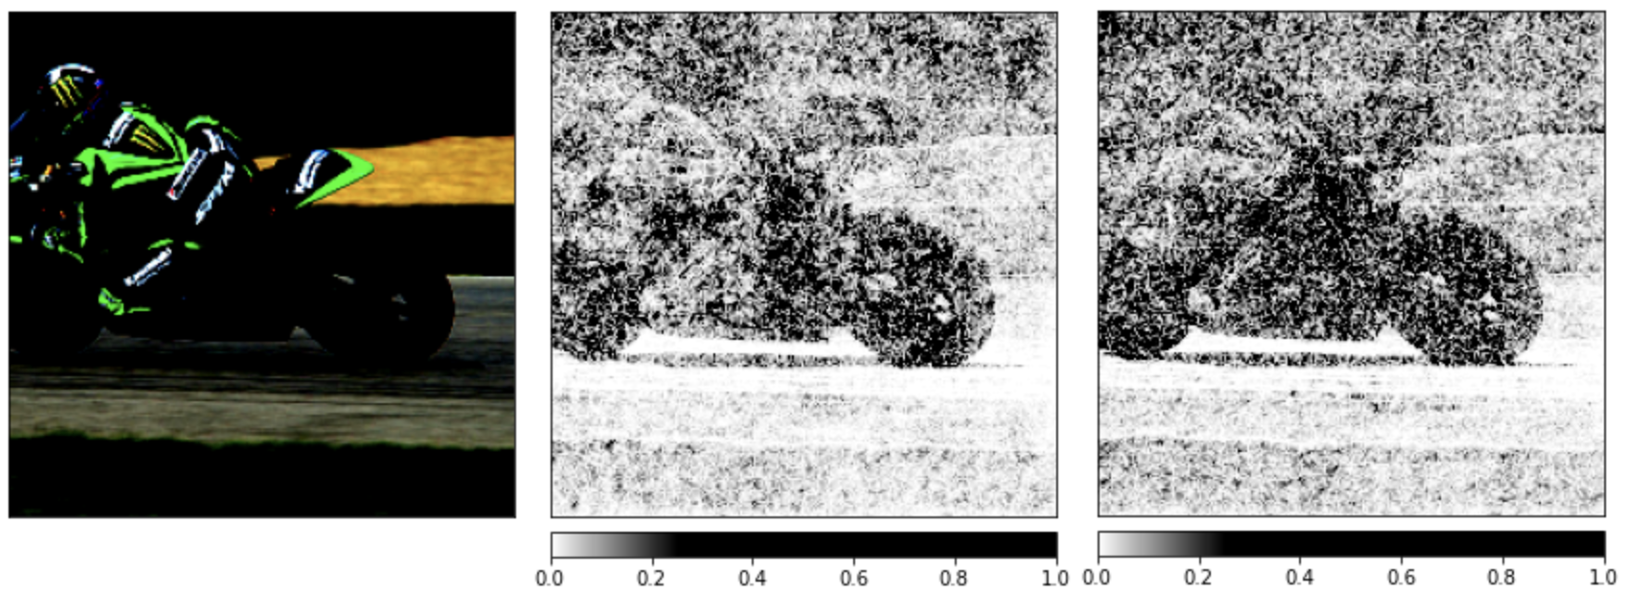
\includegraphics[width=0.9\textwidth]{figures/images.png}}
\caption{Comparison between Integrated Gradients and Geodesic IG on one image. The predicted class is ``motor-scooter". The left figure is the original image, while the other two are heatmaps of respectively the IG (center) and the Geodesic IG (right). We can see that our method seems to reduce the amount of noise and is able to provide a sharper heatmap, compared with the vanilla IG. More comparisons are presented in Appendix \ref{app:voc}.}
\label{fig:qualitative-comp}
\end{center}
\vskip -0.2in
\end{figure*}

Now we would like to test our method on a real-world dataset. To this aim, we use the Pascal VOC 2012 dataset, which consists of labelled images \citep{pascal-voc-2012}. We also use a pre-trained ResNet model to generate predictions to be explained \citep{he2016deep}. We also perform the analysis on 100 randomly sampled images from the test set.

We compare our method with various baselines: Integrated Gradients, GradientShap, SmoothGrad, InputXGradients \citep{shrikumar2016not}, Lime \citep{ribeiro2016should}, KernelShap \citep{lundberg2017unified}, Occlusion \citep{zeiler2014visualizing} Augmented Occlusion \citep{tonekaboni2020went} and Enhanced IG \citep{jha2020enhanced}.

For both Enhanced IG and Geodesic IG, as the VOC dataset is high-dimensional, we generate points of the graph following the method described in our Method section, using the straight line as a guide. The baseline is chosen here as a uniformly black image. As with the half-moons dataset, we use 5 neighbours for the kNN algorithm.

To evaluate the performance of an attribution method, we use here 3 different metrics:

\begin{itemize}
    \item \textbf{Comprehensiveness} \citep{deyoung2019eraser}: We mask the top k\% most important features in absolute value, and compute the average change of the predicted class probability compared with the original image. A higher score is better as it indicates masking these features results in a large change of predictions.
    \item \textbf{Sufficiency} \citep{deyoung2019eraser}: We only keep the top k\% most important features in absolute value, and compute the average change of the predicted class probability compared with the original image. A lower score is better as it means that these important features are sufficient to retain similar predictions.
    \item \textbf{Log-odds}\footnote{This metric should be called \emph{Log-probabilities}. However, since Log-odds is a commonly used name in the literature, we refer to it as Log-odds.} \citep{shrikumar2017learning}: We mask the top k\% most important features in absolute value, and measure the negative logarithmic probabilities on the predicted class compared with the original one. Lower scores are better.
\end{itemize}

\begin{table}[t]
	\centering
	\resizebox{0.48\textwidth}{!}{%
	\begin{tabular}{lccc}
		\toprule
		\textbf{Method} & Comp $\uparrow$ & Suff $\downarrow$ & LO $\downarrow$ \\
		\midrule
        Input X Gradients   & 0.360 (0.0280) & 0.545 (0.0254) & -2.66 (0.167)  \\
        GradientShap        & 0.425 (0.0130) & 0.544 (0.0260) & -3.28 (0.164)  \\
		IG                  & 0.427 (0.0072) & 0.544 (0.0254) & -3.31 (0.117)  \\
        SmoothGrad          & 0.404 (0.0160) & 0.536 (0.0263) & -3.09 (0.222)  \\
        Lime                & 0.197 (0.0139) & 0.529 (0.0176) & -1.31 (0.082)  \\
        Kernel Shap         & 0.193 (0.0179) & \textbf{0.527} (0.0172) & -1.30 (0.114) \\
        Occlusion           & 0.340 (0.0263) & 0.534 (0.0211) & -2.26 (0.061) \\
        Aug Occlusion       & 0.352 (0.0177) & 0.540 (0.0235) & -2.37 (0.118) \\
        Enhanced IG         & 0.445 (0.0104) & 0.543 (0.0264) & -3.75 (0.125) \\
		\midrule
		Geodesic IG         & \textbf{0.449} (0.0107) & 0.543 (0.0261) & \textbf{-3.77} (0.168) \\
		\bottomrule
	\end{tabular}%
	}
	\caption{Evaluation of different attribution methods on 100 randomly sampled images from the Pascal VOC test set. The metrics are computed by removing or keeping the top 5\% most important features. More results are provided in Appendix \ref{app:voc}.}
	\label{tab:results_voc}
\end{table}

Figure \ref{fig:qualitative-comp} provides a qualitative comparison between Geodesic IG and Integrated Gradients, while Table \ref{tab:results_voc} provides a quantitative comparison between Geodesic IG and various other methods. The analysis shows that Geodesic IG is a very powerful method in explaining the model's behavior on the dataset. Table \ref{tab:results_voc} shows that for this dataset, Geodesic IG outperforms almost all other methods in terms of comprehensiveness and log-odds, and is on par with Enhanced IG. However, as we further discuss in section \ref{sec:related_work}, the path of Enhanced IG does not take the model's gradients into account, potentially leading to significant artefacts, and lacks a straightforward way for improvement. On the other hand, Geodesic IG could be further improved by deriving better approximations of the geodesic path, which we discuss in section \ref{sec:method}. In this experiment, we have indeed used the simple `guide' method according to Eq. \ref{eq:guide}, and we expect that a more sophisticated approximation method would further improve the results.

Furthermore, the Sufficiency results in Table \ref{tab:results_voc} do not seem to discriminate between different explanation methods. However, in Appendix \ref{app:voc} we present more results, in which Geodesic IG outperforms the original IG on this metric.
